\documentclass[../main.tex]{subfiles}
\begin{document}
\section{Introduction}

Residential segregation, the uneven distribution of ethnic groups within a confined geographic area, remains a persistent feature of Danish society, yet there is limited empirical evidence on how ethnic background directly influences residential sorting. To this end, I seek to answer the fundamental question: To what extent do households respond directly to the ethnic identity of their nearest neighbors when making the decision to move?

\textcite{schelling1971dynamic} remains the foundational piece in the literature on theoretical determinants of segregation. The key prediction of \textcite{schelling1971dynamic} is that neighborhoods may experience a rapid outflow of residents belonging to a majority, or "tip", when the share of (new) residents belonging to a minority reach a certain threshold. \textcite{schelling1971dynamic} noted that this phenomenon may happen even if majority residents are relatively tolerant of other minorities.\footnote{To illustrate, I have simulated a simple version of Schelling's model, which takes inspiration from \textcite{luca_mingarelli}. This can be found in Appendix \ref{sec:appendix_schelling_model_simulation}.} This paper focuses on what Schelling called the "third" kind of segregation - individually motivated segregation - as distinct from organized segregation (such as historical Jim Crow laws) or economically induced segregation (clustering by income or education).  I do not make the claim that organized or economically induced segregation do not exist or play a role in Denmark (perhaps less so than in the United States), but that individual preferences, even if it is not the main driver of observed segregation, still matters and deserves attention. 

The Danish context offers a particularly valuable setting for this research question. Over the past four decades, Denmark has transformed from a relatively homogeneous society to one with increasing ethnic diversity, particularly in urban areas. This demographic shift, combined with Denmark's comprehensive administrative data infrastructure, provides an ideal environment to examine Schelling behavior in a European welfare state context.

Work by \textcite{schelling1971dynamic} has spawned a rich literature on segregation from which many papers draw their inspiration from. \textcite{card2008tipping} employ a single "tipping point" Schelling model in an RDD setting. They find discontinuity in the rate of change in minority shares ranging between 5 pct. (Portland, Oregon) to around 20 pct. (Los Angeles, California). Inspired by \textcite{card2008tipping}, \textcite{bohlmark_willen_2020_tipping} estimate neighborhood tipping points in Sweden's largest cities (Stockholm, Malmo and Gothenburg) that range between 17-19 pct. minority shares. \textcite{blair2017outside} further builds on \textcite{card2008tipping} and the idea of neighborhood tipping points in the United States, but points to the importance of outside options in this context. \textcite{blair2017outside} argues that while some White American households may dislike neighbors from a different ethnic background, they may be constrained by unattractive alternatives. Here, outside option refers to the set of neighboring census tracts that exists within a household's Metropolitan Statistical Area (MSA). 

While the tipping point literature has advanced our understanding of neighborhood-level dynamics, identifying the causal mechanisms underlying these patterns remains challenging. \textcite{Bayer_2022_nearest_neighbor} address this challenge by developing a nearest neighbor research that examines household responses to specific neighbor changes at precise spatial location within a neighborhood. By comparing households within the same neighborhood who receive different-type neighbors either next-door or "just down the road", they isolate preferences about neighbors from preferences about neighborhood amenities. Once applied to a US setting, they find symmetric responses among both  White and Black households, with 4-6 percent increases in baseline exit rates within 2 years following the arrival of a different-race neighbor. This paper adapts their methodological approach to a Danish context, allowing for a novel comparison of Schelling mechanisms across different institutional settings. 

Identifying the causal role of preferences for neighborhood composition is vital for understanding persistent segregation. It has been widely established that neighborhoods, both who live there and amenities within, matter for long-run outcomes. For instance, \textcite{chetty2016effects} show the positive impact on earnings and college attendance when presented with the opportunity to move to a more affluent neighborhood. In a Danish context, \textcite{hasager2024sick_poor_neighborhood} show the importance of neighborhood (both at the building and parish level) composition on long-term health outcomes using the quasi-experiment of the Danish Spatial Policy for refugee placement. \textcite{damm2014crime} use the same policy as part of their empirical framework and finds that neighborhood crime rates is strongly associated with youth criminal behavior. In an American context, \textcite{caetano2017school} argue much of the residential sorting found in the US is the result of the parental preferences for the racial and socioeconomic composition of schools, which can lead schools to "tip" with school segregation even greater than neighborhood segregation. \textcite{andreas_gandil_2024attendance_school_segregation} find similar patterns in a Danish context, where parental school preferences cause segregation in school attendance with a strong socioeconomic gradient in responses. 

Perhaps most similar to me is \textcite{rockwool_boje2024immigrants}, who examine native flight in Denmark, both at the neighborhood and building level. They find that an increase in 30 percentage points in the share of non-Western foreigners in the neighborhood increase the propensity for natives to move out in any given year by around 8 pct.\footnote{Neighborhoods contain around 600 households in \textcite{rockwool_boje2024immigrants}. These are derived from work by \textcite{damm2008danish}.} Unlike these previous studies that often rely on neighborhood-level data, I leverage a unique administrative dataset that pinpoints individual residential locations with precise spatial coordinates and exact timing of moves. Using this granular data, I implement the nearest neighbor research design developed by \textcite{Bayer_2022_nearest_neighbor}, comparing households within the same neighborhood who receive different-type neighbors either next-door or just down the road. I focus specifically on interactions between native and non-Western households to test for potential asymmetry in Schelling behavior, extending previous work by examining these dynamics in the context of a European welfare state.

I find that native Danish household increase their propensity to move within 2 years by approximately 0.3 percentage points, an increase by 1.6 percent compared to their baseline exit rate, when they receive a new non-Western neighbor among their three nearest neighbors compared to "just down the road". This effect is robust across specifications and primarily driven by low-SES native households responding to low-SES non-Western neighbors. In contrast, non-Western households do not show the same type of behavior for new native neighbors, which highlights the asymmetry in Schelling behavior in Denmark.  

The paper is structured as follows. Section \ref{sec:model} presents the theoretical framework and empirical strategy heavily influenced by \textcite{Bayer_2022_nearest_neighbor}. Section \ref{sec:data} describes the data sources, the steps taken to process the unique datasets used in this paper along with descriptive statistics on neighborhood composition. In section \ref{sec:results}, I show my main results and heterogeneity in Schelling behavior. I conclude on my findings in section \ref{sec:conclusion}.

\subsection{Definitions}
\label{sec:intro_definitions}
In the paper, I define 3 mutually exclusive types of households. (i) \textit{Native} households, where all members are of Danish origin; (ii) \textit{non-Western} households, where at least one member is of non-Western origin and (iii) \textit{Western} households, where at least one household member is non-Native and of Western origin, but with no members that have \textit{non-Western} origin. I follow the definition of Western/non-Western countries by \textcite{west_non_west_def_dst}.\footnote{Throughout the paper, I repeatedly write about "same"- and "different"-type neighbors. To be clear, same-type neighbors refers to two or more households that live in close proximity to each other and both fall within the same category defined above. If they differ in terms of household type, they are different-type neighbors.}

\end{document}







% 1) Determine treat/control
% - Treat: New non-West among K=3
% - Control: New non-west among K=4,..,40? 
% - Drop everyone else
% 2) Make panel. use lf.join_where(pl.date_range(..., eager=True)
% 3) Take unique ID's and collect
% - Inc, edu, emp
% 4) just have a little looksy @ BBR / DAR

%Section \ref{sec:model} outlines and  simulates a simplified of the Schelling model. Section \ref{sec:data} describes the data used in this paper. The empirical strategy is presented in Section \ref{sec:empirical_strategy}. The main results, including a heterogeneity analysis (?), are presented in Section \ref{sec:results}. In Section \ref{sec:Discussion}, I discuss some stuff(?). In Section \ref{sec:conclusion} I summarize and conclude.
Cont...

Include some stats:

\begin{figure}[H]
\centering
\caption{Different-type neighbors}
    \begin{subfigure}{0.47\textwidth}	
	\centering
    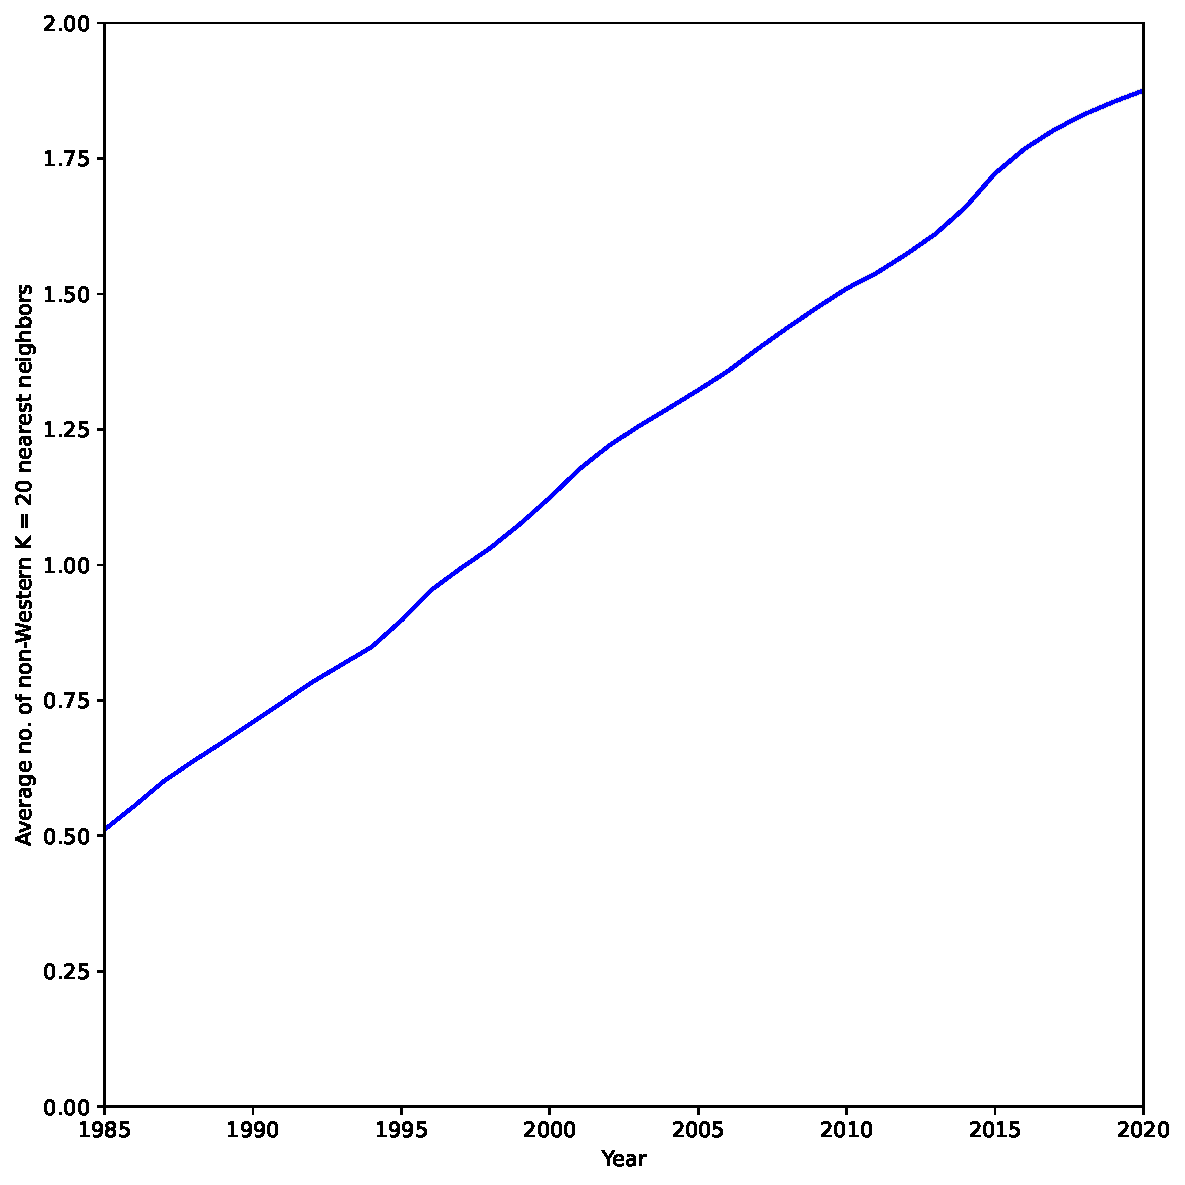
\includegraphics[width=\linewidth]{figs/mix_non_west_pos_nn_1985_2020.pdf}
	\caption{Non-Western neighbors} 
	\end{subfigure}	
    \begin{subfigure}{0.47\textwidth}	
	\centering
    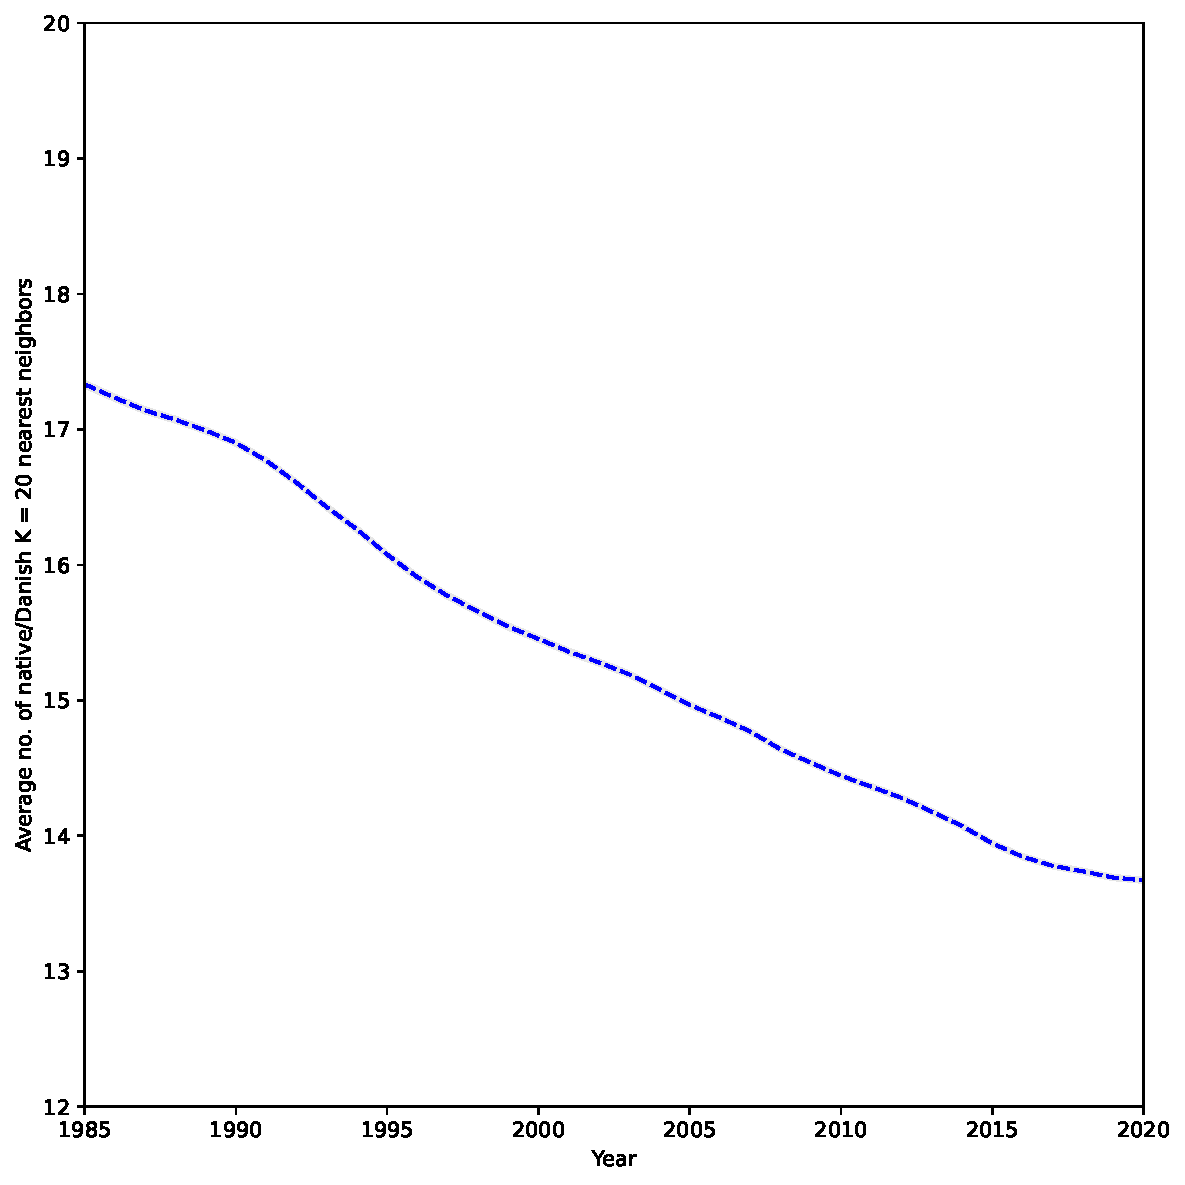
\includegraphics[width=\linewidth]{figs/native_nn_1985_2020.pdf}
	\caption{Danish/native neighbors} 
	\end{subfigure}	
      
    \label{fig:avg_k_nearest_dk}
    \begin{minipage}{.9\linewidth}
        \footnotesize \textit{Note}: Non-Western households refers to households where at least one household member is of non-Western origin. Danish/native households refers to households where all members is of Danish descent.
    \end{minipage}
\end{figure}

Some figures yet to be determined where to place can be found in Appendix \ref{sec:appendix_figs}
